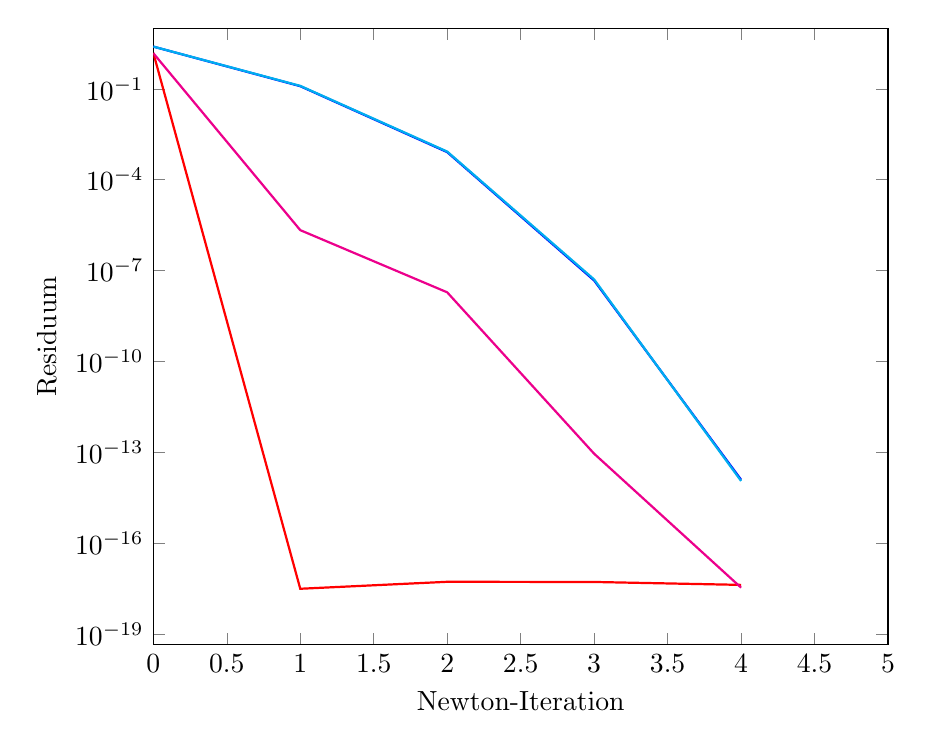
\begin{tikzpicture}[every plot/.append style={thick}] 
\begin{axis}[ 
label style={font=\normalsize}, 
xlabel={Newton-Iteration}, 
ylabel={Residuum}, 
xmin=0, xmax=5, 
ymode=log, 
ymin=0, ymax=10, 
width=0.9\textwidth, 
grid style=dashed, 
] 
\addplot[ 
color=blue, 
] 
coordinates { 
(0, 2.47e+00)(1, 1.22e-01)(2, 8.10e-04)(3, 4.68e-08)(4, 1.23e-14)}; 
\addplot[ 
color=red, 
] 
coordinates { 
(0, 1.54e+00)(1, 3.09e-18)(2, 5.25e-18)(3, 5.18e-18)(4, 4.15e-18)}; 
\addplot[ 
color=cyan, 
] 
coordinates { 
(0, 2.48e+00)(1, 1.25e-01)(2, 8.46e-04)(3, 5.06e-08)(4, 1.12e-14)}; 
\addplot[ 
color=magenta, 
] 
coordinates { 
(0, 1.50e+00)(1, 2.15e-06)(2, 1.90e-08)(3, 8.90e-14)(4, 3.36e-18)}; 
\end{axis} 
\end{tikzpicture} 
